\chapter{La Cybersécurité et La Sécurité Informatique}
\section{La Cybersécurité}
\subsection{Définition}

La racine « \textbf{cyber} » provient du mot cybernétique, qui avait été formé en français
en 1834 pour désigner la «\textbf{ science du gouvernement} », à partir du grec Kubernêtiké, signifiant « \textbf{diriger, gouverner} ».\\
Terme repris en 1948, par le mathématicien Norman Wiener aux États-Unis à l’origine de la cybernétique (cybernetics), science constituée par l’ensemble des théories relatives au contrôle, à la régulation et à la communication entre l’être vivant et la machine.\\
La cybersécurité, également appelée sécurité informatique ou sécurité des technologies de l'information, est l'ensemble des mesures techniques, organisationnelles et juridiques mises en place pour protéger les systèmes informatiques, les réseaux et les données contre les attaques, les pertes ou les altérations.\\
 Elle vise à garantir la confidentialité, l'intégrité et la disponibilité des informations stockées sur les systèmes informatiques, ainsi que la protection de la vie privée et des droits de propriété intellectuelle.\\

La cybersécurité concerne la sécurité informatique et des réseaux des environnements connectés à Internet et accessibles via le cyberespace.\\
 Elle peut être mise en défaut, entre autres, par des cyberattaques informatiques.\\
 Du fait de l’usage extensif d’Internet, de nouvelles menaces sont apparues générant des risques additionnels dont les impacts, de niveaux d’importance variables, peuvent affecter les individus, les organisations ou les États.\\ 

La cybersécurité est devenue un enjeu majeur dans le monde numérique d'aujourd'hui, où les attaques informatiques sont de plus en plus sophistiquées et fréquentes.\\
 Elle est essentielle pour protéger les systèmes informatiques et les données sensibles contre les menaces potentielles et assurer la continuité des activités des organisations qui les utilisent.\\
  La cybersécurité est également importante pour protéger les utilisateurs finaux, tels que les consommateurs et les employés, contre les risques de vol d'identité, de fraude en ligne et d'autres formes de cybercriminalité.\\
Le préfixe « Cyber » est relatif à l’environnement informatique et aux activités
rendues possibles par les technologies du numérique et de l’Internet.\\
 Le cyberespace (l’ensemble des infrastructures numériques, des données et des services mis en réseaux) est une extension de notre espace naturel qui reflète notre société avec ses réalités politique, économique, sociale et culturelle.\\
  Mais contrairement à la terre, à la mer, à l’air et à l’espace-extra atmosphérique, le cyberespace est une pure création de l’être humain qui ne relève pas de la nature.\\

Les points essentiels englobés par la cybersécurité comprennent :
\space 
 
 \paragraph{1. La confidentialité :\\}la protection des données contre les accès non autorisés. Cela inclut la protection des données personnelles, des secrets commerciaux, des informations financières et autres informations sensibles.

 \paragraph{2. L'intégrité :\\}  la protection des données contre les altérations non autorisées. Cela inclut la garantie que les données sont exactes et fiables.

 \paragraph{3. La disponibilité :\\}  la garantie que les systèmes, les réseaux et les données sont accessibles et fonctionnent correctement, et que les interruptions de service sont minimisées.

 \paragraph{4. L'authenticité:\\} la garantie que les utilisateurs sont bien ceux qu'ils prétendent être, et que les données sont bien celles qu'elles prétendent être.

 \paragraph{5. La non-répudiation:\\} la garantie qu'une personne ne peut pas nier avoir effectué une action ou avoir envoyé des données.

 \paragraph{6. La résilience :\\} la capacité des systèmes et des réseaux à résister aux attaques et à récupérer rapidement en cas d'incident.


 \paragraph{7. La conformité :\\} le respect des lois, des réglementations et des normes en matière de sécurité informatique.

 \paragraph{8. La sensibilisation :\\} l'éducation et la formation des utilisateurs pour qu'ils comprennent les risques liés à la sécurité informatique et les meilleures pratiques à suivre pour les éviter.
 
Ces points essentiels sont inter-connectés et doivent être pris en compte dans toute stratégie de cybersécurité efficace.\\
\subsection{Pourquoi la cybersécurité est-elle nécessaire ?}
En 2021, le cybercrime a coûté au monde 6 000 milliards de dollars américains. D’ici 2025, ce coût passera à 10500 milliards de dollars.\\
 Le cybercrime est un problème de plus en plus sérieux, et pour s’y attaquer, il est essentiel de disposer d’un excellent dispositif de cybersécurité.\\

Les individus, les gouvernements, les entreprises, les organismes à but non lucratif et les établissements d’enseignement risquent tous de subir des cyberattaques et des violations de données.\\
 À l’avenir, le nombre d’attaques se multipliera, avec l’évolution des technologies numériques, l’augmentation du nombre d’appareils et d’utilisateurs, les chaînes logistiques mondiales de plus en plus complexes, et le rôle de plus en plus stratégique des données dans l’économie numérique.\\
  Pour minimiser le risque d’une attaque et pour sécuriser les systèmes et les données, un solide dispositif de cybersécurité devient vital.\\
\subsection{Comment les risques de cybersécurité sont-ils mesurés ?}
Le risque de cybersécurité correspond au potentiel de perte ou de préjudice résultant de l’endommagement d’une ressource informatique, susceptible d’entraîner un vol de propriété intellectuelle, une perte financière, une atteinte à la réputation, et des amendes légales ou réglementaires. En mesurant les risques, les entreprises peuvent optimiser les actions permettant de mieux les gérer, et s’assurer ainsi qu’il n’y a pas d’obstacles aux objectifs commerciaux.\\

\textbf{Identifier les ressources et définir leur priorité.} L’évaluation des risques de cybersécurité commence par la compréhension des ressources de l’entreprise et la définition de leur priorité, en établissant celles dont la perte, l’exposition ou l’endommagement pourrait avoir un impact sur les opérations.\\

\textbf{Identifier les vulnérabilités.}
 Toutes les vulnérabilités susceptibles de laisser une menace causer des dommages sont identifiées à l’aide de l’analyse automatique des vulnérabilités, des tests d’intrusion, ou de l’utilisation d’une base de données de vulnérabilités telle que la  \href{https://nvd.nist.gov/}{base de données nationale des vulnérabilités du NIST.}\\
 
 \textbf{Calculer l’impact de la menace.} L’impact probable ou le dommage que pourrait causer une menace à une ressource est calculé et classé comme élevé, moyen ou faible.\\
 \textbf{Calculer le risque.}Risque = Menace x Vulnérabilité x Ressource. À partir de cette équation, l’entreprise peut mesurer chaque risque.\\
\textbf{ Créer une matrice de risques pour la planification des corrections.} Enfin, la matrice de risques est établie, les deux axes représentant la probabilité et l’impact.\\

\textbf{Risque = Probabilité x Impact.} À partir de cette valeur, chaque risque est classé comme élevé, moyen ou faible, à la suite de quoi les stratégies de réduction appropriées sont mises en œuvre.\\
	
	 
	 
\begin{figure}[h]
	\begin{center}
	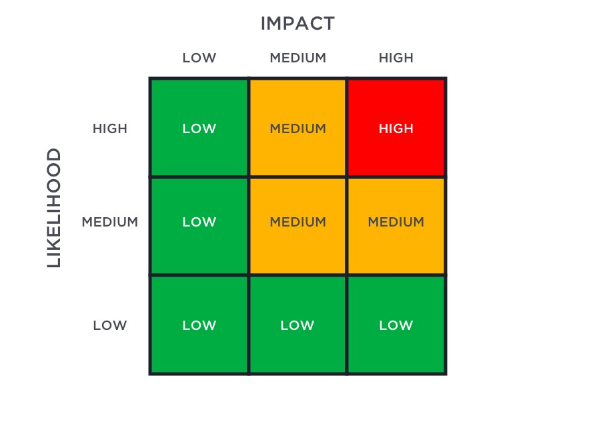
\includegraphics[width=0.7\textwidth]{PhotoMemoire/tableauImpact.png}
\caption{Un Tableau Illustrant Les Impact \cite{15}}
\end{center}
\end{figure}

\subsection{Cybersécurité avfondeur (DEP)}
Il n’existe pas de méthode ou d’outil de cybersécurité capable de défendre de tous les types d’attaque. Voilà pourquoi la cybersécurité avec défense en profondeur (DEP) est essentielle.\\
Avec la DEP, également connue sous le nom d’ « approche forteresse » en matière de cybersécurité, des mécanismes défensifs multiples sont mis en œuvre pour protéger les ressources d’entreprise.\\
Cette approche multicouche renforce la sécurité globale. De plus, si un mécanisme échoue, les autres fonctionneront pour prévenir ou stopper les cyberattaques.\\

Une stratégie de cybersécurité avec DEP inclut différents éléments :\\

\textbf{Logiciel antivirus.} 
Les solutions antivirus comportant des fonctionnalités heuristiques qui recherchent et signalent les activités suspectes offrent une plus forte protection que les solutions classiques basées sur des signatures.\\

\textbf{Contrôles de sécurité du réseau.} 
Les pare-feu et les systèmes de protection contre les intrusions peuvent identifier des menaces de sécurité potentielles, et les bloquer à partir de règles de sécurité.\\

\textbf{Solutions d’intégrité des données.}
Ces produits vérifient les adresses IP sources pour confirmer que les fichiers entrants proviennent de sources connues et de confiance uniquement.\\

	\textbf{Analyse comportementale.} Ces systèmes analysent les comportements des fichiers et des réseaux en fonction de comportements « normaux » prédéfinis.\\
		Ils envoient ensuite des alertes ou effectuent des actions automatiques pour bloquer une violation ou l’empêcher de se poursuivre.\\
		
	\textbf{Stratégies et procédures.} Les stratégies de gestion des risques, de gestion de la chaîne logistique, de la réponse aux incidents, etc. permettent de renforcer la cybersécurité.\\
\begin{figure}[h]
\begin{center}
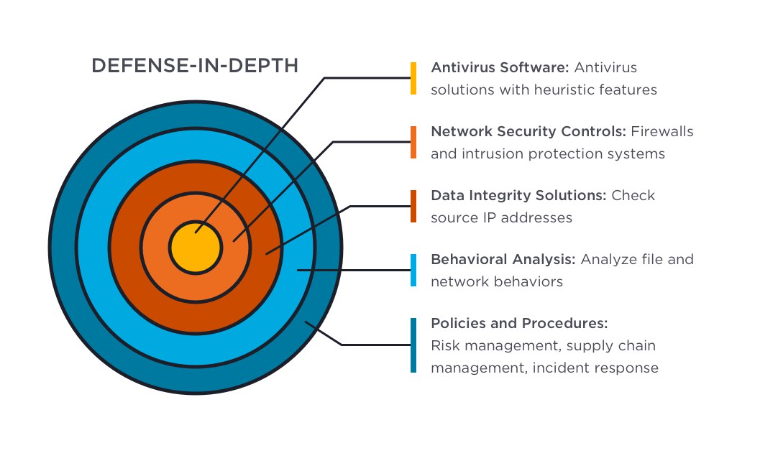
\includegraphics[width=0.8\textwidth]{PhotoMemoire/dep_image.png}
\caption{Un Schéma Illustrant Le DEP \cite{15} }
\end{center}
	\end{figure}
	
	
	
	\pagebreak
	\newpage
	\subsection{Comment mettre en œuvre laec déen pro cybersécurité}
 Le panorama des cybermenaces est en constante évolution. La mise en œuvre d’un solide dispositif de cybersécurité peut donc s’avérer être un véritable défi. Elle n’est toutefois pas impossible,\\
  si les entreprises suivent une approche systématique en intégrant les éléments suivants :
  
  \textbf{Analyse et gestion des risques.} Une approche basée sur les risques garantit que les équipes de sécurité auront connaissance des risques les plus critiques pour l’entreprise, et pourront adopter l’intervention adéquate pour réduire leur impact éventuel.\\
  \textbf{Inventaire et gestion des ressources.} Il est essentiel de comprendre les ressources d’une entreprise pour appréhender et gérer les risques qui menacent ces ressources.
  Identification et gestion des vulnérabilités.\\ Les vulnérabilités doivent être identifiées et corrigées dès que possible, en particulier si elles sont critiques et peuvent véritablement nuire à l’entreprise.\\
  
  \textbf{Déploiement de la gestion des accès et identités.} Pour éviter à la fois les attaques de l’intérieur et de l’extérieur, il est essentiel de protéger et de contrôler l’accès aux services, aux systèmes et aux données.
  
  \textbf{Sécurité des données.} L’ensemble des données organisationnelles doit être protégé de tout accès ou utilisation non autorisés.\\
  
  \textbf{Gestion des incidents.} Une bonne gestion des incidents peut réduire l’impact et les dommages causés par les incidents de sécurité.\\
  
  \textbf{Sécurité de la chaîne logistique.} Il est essentiel d’identifier et d’appréhender de manière cohérente les risques et vulnérabilités sur les réseaux tiers.\\
  
  \textbf{Formation des salariés.} Selon une étude IBM, l’erreur humaine est responsable de 49 pourcent  des violations. Une autre étude de la Stanford University estime que les erreurs humaines, en particulier celles des salariés, est à l’origine de 88 pourcent des violations. Les salariés utilisent souvent des mots de passe faibles, se font avoir par les e-mails d’hameçonnage, ou n’installent pas les mises à jour de sécurité sur leurs appareils. Il est vital de former le personnel aux bonne habitudes de cybersécurité pour bénéficier d’une solide protection.\\
  \paragraph{ }
  L’identification, l’évaluation et la mesure des risques sont des composantes importantes de la mise en place d’un programme de cybersécurité. Sans ces étapes essentielles, les entreprises ne pourront sans doute pas mettre en œuvre un dispositif solide, ni améliorer leur posture de sécurité.
  \begin{figure}[h]
  	 \begin{center}
  	 		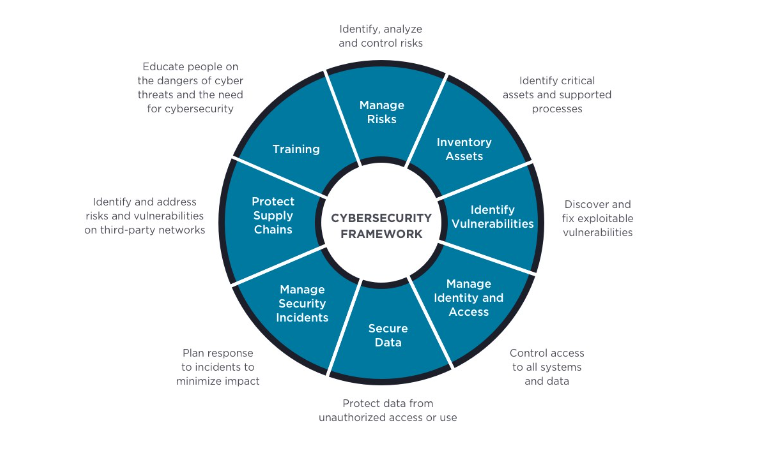
\includegraphics[width=0.8\textwidth]{PhotoMemoire/image_oeuvre.png}
  	 		\caption{Le CyberSecurity Framework \cite{15} }
  	 \end{center}
  \end{figure}
  
 \section{But}
 Le but concret de la cybersécurité est de protéger les systèmes informatiques, les réseaux, les programmes et les données contre les attaques, les dommages, les modifications ou les fuites non autorisées. La cybersécurité vise à prévenir les cyberattaques, à détecter les violations de sécurité, à réduire les dommages potentiels et à réagir efficacement en cas d'incident de sécurité.\\
 \section{objectif}
 L'objectif concret de la cybersécurité est de protéger les systèmes informatiques, les réseaux, les programmes et les données contre les attaques, les dommages, les modifications ou les fuites non autorisées. La cybersécurité vise à prévenir les cyberattaques, à détecter les violations de sécurité, à réduire les dommages potentiels et à réagir efficacement en cas d'incident de sécurité.\\
 \paragraph*{ }
 En 2020, le vol de données et les cyberattaques arrivaient à la 6e et à la 7e place des risques mondiaux les plus importants en termes de probabilité de survenue.\\ En 2021, les hackers continuent d’exploiter la pandémie de COVID-19 et le passage au télétravail opéré en conséquence.\\ Ainsi, les cyberattaques ont augmenté de 21 pourcent dans le monde entier. La cybersécurité joue un rôle crucial pour se tenir à distance de telles menaces et des personnes malveillantes.\\
 
 Les cybercriminels recherchent constamment le talon d’Achille des systèmes informatiques d’entreprise.\\ Pour éviter d’être victimes de cyberattaques, les entreprises doivent mettre en œuvre les outils, les technologies et le personnel adéquats en matière de cybersécurité.\\
\section{La Sécurité Informatique}
\subsection{Définition}
 La sécurité informatique est l'ensemble des mesures techniques, organisationnelles et juridiques mises en place pour protéger les systèmes informatiques, les réseaux et les données contre les attaques, les pertes ou les altérations. Elle vise à garantir la confidentialité, l'intégrité et la disponibilité des informations stockées sur les systèmes informatiques, ainsi que la protection de la vie privée et des droits de propriété intellectuelle. \\

 La sécurité informatique englobe un large éventail de domaines, tels que la sécurité des réseaux, la sécurité des systèmes d'exploitation, la sécurité des applications, la sécurité des données, la sécurité physique, la gestion des identités et des accès, la conformité aux normes de sécurité, la surveillance et la détection des incidents de sécurité, ainsi que la réponse aux incidents de sécurité.\\

  La sécurité informatique est devenue un enjeu majeur dans le monde numérique d’aujourd’hui, où les attaques informatiques sont de plus en plus sophistiquées et fréquentes. La mise en place d'une politique de sécurité informatique efficace est donc essentielle pour protéger les systèmes informatiques et les données sensibles contre les menaces potentielles et assurer la continuité des activités des organisations qui les utilisent.\\
\begin{figure}[h]
	\begin{center}
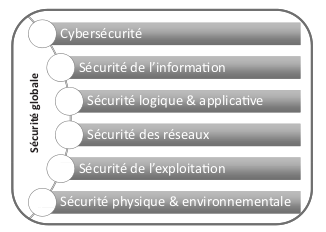
\includegraphics[width=0.5\textwidth]{PhotoMemoire/image_sec.png}
\caption{Les Différents Points Englobés par La sécurité Informatique \cite{15}}
	\end{center}
\end{figure}

La sécurité informatique englobe plusieurs domaines d'applications :
\begin{enumerate}
\item  sécurité physique et environnementale ;
\item  sécurité de l’exploitation ;
\item   sécurité des réseaux ;
\item  sécurité logique, sécurité applicative 
\item   sécurité de l’information ;
\end{enumerate}
Dans Le cas de notre Serveur Web nous allons voir quels sont les impacts que les différents domaines d'application ont. \\ 
\section*{Sécurité physique et environnementale }
La sécurité physique est souvent définie comme la protection du personnel, du matériel, des logiciels, des réseaux et des données contre les actions physiques et les événements qui pourraient causer des pertes ou des dommages graves à une organisation.\\
La sécurité physique est une pratique commerciale d'une importance vitale avec de nombreux objectifs : empêcher les personnes non autorisées d'entrer dans une entreprise et de causer des dommages ; protéger la propriété intellectuelle contre l'espionnage des entreprises ; et atténuer la violence sur le lieu de travail, entre autres préoccupations.\\
 Aujourd'hui, les organisations doivent considérer la sécurité physique comme un pilier principal de leur stratégie de cybersécurité.\\
 Le succès du programme de sécurité physique d'une organisation peut souvent être attribué à la façon dont chaque composante est mise en œuvre, améliorée et maintenue.\\

\section*{Sécurité de L'information} 
 La sécurité de l'information (infosécurité, infosec) est un ensemble de stratégies de gestion des processus et politiques visant à protéger, détecter, recenser et contrer les menaces ciblant les informations numériques ou non.\\
 Parmi ses responsabilités, l'infosécurité doit établir un ensemble de processus d'entreprise qui protègeront les actifs informationnels indépendamment du format ou de l'état des informations (en transit, en cours de traitement ou stockées au repos).\\
 
 \section*{Sécurité Logique et Applicative}
 La sécurité logique complète la sécurité physique. Sa fonction est de protéger les systèmes, processus et programmes de protection des logiciels et des données, ainsi que l’accès ordonné et autorisé des utilisateurs aux informations.\\
  La sécurité logique comprend toutes les mesures établies par la direction pour minimiser les risques de sécurité associés aux opérations quotidiennes effectuées à l’aide des technologies de l’information, comme le vol d’information, la perte de données, l’entrée de virus, la modification non autorisée de données, les attaques de réseaux, etc.\\
   La sécurité logique vise à préserver la confidentialité, l’intégrité, l’authenticité et la disponibilité des données.\\
 
 La sécurité applicative quant a elle  concerne la manière dont les applications sont développées pour garantir qu'elles sont sécurisées. Elle comprend des mesures de sécurité telles que la validation des entrées, la gestion des erreurs, la gestion des sessions, la gestion des cookies, la protection contre les injections SQL, la protection contre les attaques de script et la protection contre les attaques de force brute. La sécurité applicative vise également à garantir que les applications sont développées selon des normes de sécurité élevées afin de prévenir les vulnérabilités et les failles de sécurité.\\
 
 L’ère numérique a forcé les entreprises à accorder plus d’attention à leur bien le plus précieux: l’information. Aujourd'hui, investir dans la sécurité informatique est vital pour la protection des données de toute organisation. Si vous souhaitez sécuriser vos informations et les protéger contre les attaques, demandez conseil à des experts professionnels en sécurité informatique.
 
 \section*{Sécurité Des Réseau}
 Dans l'infrastructure informatique moderne de l'entreprise, les données sont autant susceptibles d'être en mouvement qu'au repos.\\
  C'est là qu'intervient la sécurité réseau. Si elle fait techniquement partie de la cybersécurité, la sécurité réseau concerne surtout l'infrastructure réseau de l'entreprise.\\
   Elle gère différents aspects notamment la sécurisation de la périphérie du réseau ; les mécanismes de transport des données (commutateurs, routeurs) ; et les dispositifs technologiques qui protègent les données à mesure qu'elles progressent d'un nœud à l'autre.\\
    La principale différence entre cybersécurité et sécurité réseau tient à la mise en œuvre de la planification de la sécurité.\\
    Un plan de cybersécurité sans plan de sécurité réseau est incomplet ; mais un plan de sécurité réseau se suffit à lui-même.\\
 
 \section*{Sécurité de l'exploitation}
 
 L’objectif de la sécurité liée à l’exploitation est de s’assurer que le traitement de l’information est fait de façon correcte et sécurisé. Pour cela, il convient de créer, documenter et diffuser des procédures d’exploitations.
 
 Il est nécessaire de séparer les environnements de tests et d’exploitations afin de réduire les risques sur ce dernier.
 
 \paragraph{La sécurité de l’exploitation c’est aussi :\\}
 \textbf{Un SOC (Security Opérations Center).} Véritable tour de contrôle de la sécurite, le SOC centralise,analyse et répond aux incidents.\\
 
 \textbf{Un SIEM (Security Information and Event Manager).} Le SIEM collecte des informations de l’infrastructure, des systèmes, des applications afin de détecter les attaques.\\
 
\textbf{Le Threat Intelligence ou Cyber Threat Intelligence (CTI)}, est une sorte de profilage de la menace et de l’attaquant permettant une anticipation des attaques.\\
 
 \textbf{Un Tableau de bord (Dashboard)} participe à couvrir les éléments de base de la sécurité à partir d’informations collectées par les équipements de sécurité.\\
 
\textbf{La réponse à incident.} Une fois l’incident survenu il convient de pouvoir y répondre suivant une stratégie établie en amont.\\
 
 \textbf{L’Analyse Forensique} exploite les traces laissées lors d’une attaque afin de connaitre le mode opératoire et éventuellement les utiliser en justice.\\
 
\textbf{La surveillance continue ou ISCM (Information Security Continuous Monitoring)}.
 Elle s’appuie sur d’autres outils comme un SIEM ou un gestionnaire de journaux d’événements. Le but est d’évaluer le niveau de sécurité de l’entreprise et l’évolution du risque en temps réel.\\
 
 \section{La sécurité informatique, pour quoi faire ?}
 La dernière décennie a été marquée par la migration de pratiquement tous les aspects des activités d’une entreprise vers un environnement en ligne. Dès lors, chaque entreprise se retrouve exposée à un risque de cyberattaque, dont le but peut être de voler des informations sensibles, telles que des données clients et des détails de paiement, des éléments de propriété intellectuelle et des secrets commerciaux, ou tout simplement de porter atteinte à la réputation de l’entreprise.\pagebreak

 Par ailleurs, la généralisation du télétravail, la migration vers le cloud et la prolifération des appareils connectés offrent aux pirates informatiques et autres cybercriminels des possibilités quasi infinies d’attaques. Cette surface d’attaque élargie, combinée à la sophistication croissante des cyberadversaires numériques, a imposé aux entreprises de renforcer et d’actualiser leurs pratiques de sécurité afin de protéger leurs ressources basées dans le cloud en particulier.\\
 
 Dans une certaine mesure, la sécurité informatique est une question de droit. En effet, dans certains pays, la loi impose aux entreprises d’investir dans le développement et l’implémentation de concepts de sécurité informatique, tandis que d’autres pays ont fixé des normes strictes en matière de confidentialité et de protection des données.\\
 \section{Types de sécurité informatique}
 \paragraph{ }
 La sécurité informatique est un terme générique qui désigne tout plan, mesure ou outil destiné à protéger les ressources numériques d’une entreprise. La sécurité informatique comprend plusieurs éléments :\\
 
 \textbf{La cybersécurité} a pour but d’assurer la protection des ressources numériques (réseaux, systèmes, ordinateurs, données, etc.) contre les cyberattaques.\\
 
 \textbf{La sécurité des endpoints, ou protection des endpoints,} est l’approche qui vise à protéger les endpoints (ordinateurs de bureau, ordinateurs portables, terminaux mobiles, etc.) contre les activités malveillantes.\\
 
 \textbf{La sécurité du cloud} regroupe la stratégie et les solutions de protection contre les cybermenaces de l’infrastructure cloud, ainsi que de tout service ou application hébergé dans l’environnement cloud.\\
 
 \textbf{La sécurité des applications} couvre toutes les mesures mises en place pour réduire la vulnérabilité des applications et ainsi empêcher tout vol, fuite ou compromission de données ou de code au sein de l’application.\\
 
 \textbf{La sécurité du réseau }désigne les outils, les technologies et les processus utilisés pour protéger le réseau et l’infrastructure critique contre les cyberattaques et les activités malveillantes. Elle inclut un ensemble de mesures préventives et défensives conçues pour refuser tout accès non autorisé aux ressources et aux données.\\
 
 \textbf{La sécurité des conteneurs} est le processus continu de protection des conteneurs, y compris du pipeline des conteneurs, de l’infrastructure de déploiement et de la supply chain, contre les cybermenaces.\\
 
 \textbf{La sécurité de l’IoT} est une subdivision de la cybersécurité qui couvre la protection, la surveillance et la neutralisation des menaces ciblant l’Internet des objets (IoT) et le réseau de terminaux IoT connectés qui collectent, stockent et partagent des données via Internet.\\
 \section{Sécurité informatique et sécurité des informations, quelle différence ?}
 
 Bien que la sécurité informatique soit parfois confondue avec la sécurité des informations, il s’agit de deux concepts bien distincts. La principale différence réside dans la forme dans laquelle les données sont stockées et, par extension, dans la manière dont elles sont protégées.\\
 
 La sécurité des informations consiste à protéger les données, quelle que soit leur forme. Il peut s’agir de protéger les données stockées par voie électronique, ainsi que de mesures de sécurité physiques telles que le verrouillage des armoires de classeurs ou des clés d’accès aux bureaux.\\
 
 La sécurité informatique concerne quant à elle la protection des données et autres ressources exclusivement sous forme numérique.\\
 \section{Sécurité informatique et cybersécurité, quelle différence ?}
 l importe également de faire la distinction entre sécurité informatique et cybersécurité.\\
 
 La cybersécurité fait référence à la protection de l’entreprise contre tout accès non autorisé et toute attaque malveillante.\\
 
 Par comparaison, la sécurité informatique revêt un caractère plus large. Elle couvre notamment toute fonctionnalité permettant de protéger et de préserver la confidentialité, l’intégrité et la disponibilité des données contre toute menace numérique.\\ Cela peut notamment inclure la protection contre les problèmes de sécurité non malveillants en soi, comme un composant matériel défaillant ou une configuration incorrecte du système.\\
 \section{Risques associés à la sécurité informatique}
 Les risques associés à la sécurité informatique peuvent être divisés en deux catégories : les perturbations du système et les attaques malveillantes ciblées.\\
 
 Une perturbation du système peut consister en une interruption temporaire des activités de l’entreprise induite par un composant système tel qu’un composant matériel défectueux, une panne réseau ou une faille logicielle. Face à une telle situation, l’entreprise s’expose à des pertes de revenus résultant de son incapacité à fonctionner ou de l’atteinte possible à sa réputation.\\
 
 Si la préservation du fonctionnement du système constitue une composante majeure de la sécurité informatique, la protection contre les cyberattaques est plus importante encore dans la mesure où la plupart de ces attaques visent à accéder à des données ou autres informations sensibles ou à les dérober. Voici quelques cyberattaques courantes dans Les 2 Tableaux Ci-après :
 
 
    \textbf{Tableau De Cyber Attaques}
   \begin{table}[h]
 		\begin{center}
 		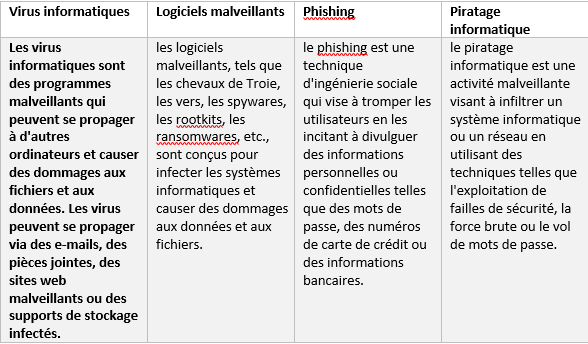
\includegraphics[width=0.7\textwidth]{PhotoMemoire/tableau1_attaques.png}
 		\caption{Tableau 1  Des Attaques}
 		  \end{center}
  \end{table}
 \vspace{2 cm}
 	\begin{table}[h]
 		\begin{center}
 		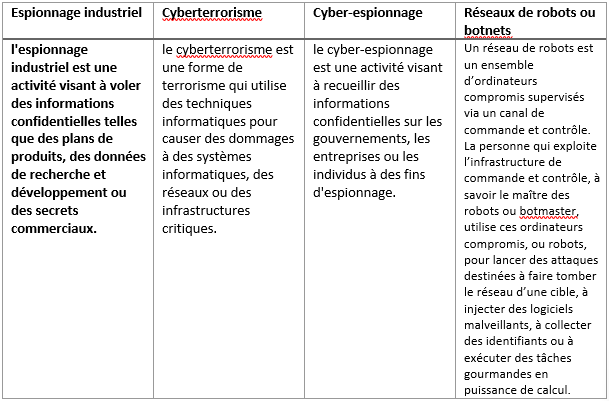
\includegraphics[width=0.7\textwidth]{PhotoMemoire/tableau2_attaques.png}
 		\caption{Tableau 2  Des Attaques}
 		 \end{center}
 	\end{table}
 
\section*{\textbf{Une stratégie de sécurité IT doit intégrer les éléments suivants :}}

\begin{itemize}
	\item[$\bullet$]\textbf{La détection et l’intervention sur les endpoints (EDR)} forment une solution complète qui identifie et contextualise toute activité malveillante afin d’aider l’équipe de sécurité à prioriser les efforts de réponse et de correction en cas de compromission de sécurité.\\
	
	\item[$\bullet$]\textbf{La détection et l’intervention managées (MDR)} sont un service de cybersécurité qui allie technologie et expertise humaine pour mettre en place des opérations de Threat Hunting, de surveillance et d’intervention. La MDR a pour principal avantage de favoriser une identification rapide des cybermenaces et d’en limiter les répercussions sans avoir à augmenter les effectifs.\\
	
	\item[$\bullet$]\textbf{La réponse à incident} consiste en une série d’étapes mises en place pour prévenir, détecter et bloquer les compromissions de données, ainsi que pour restaurer les systèmes. Elle aboutit généralement à l’établissement d’un plan de réponse à incident qui décrit les étapes et procédures que l’organisation devra suivre en cas d’incident de sécurité.\\
	
	\item[$\bullet$]\textbf{Un antivirus de nouvelle génération (NGAV, Next-Generation Antivirus)} combine intelligence artificielle, détection des comportements, algorithmes de Machine Learning et atténuation des exploits, afin d’anticiper et de prévenir immédiatement toutes les menaces de sécurité, connues comme inconnues.\\
	
	\item[$\bullet$]\textbf{Un test d’intrusion} consiste en une simulation d’attaque réelle visant à tester les capacités de détection et de réponse de l’entreprise.
	
   
\end{itemize}
\section*{Qu’attendre d’une antivirus de nouvelle génération ?}


Un antivirus de nouvelle génération efficace doit s’appuyer sur des technologies innovantes pour faire face à des cyberadversaires qui changent constamment de tactiques, techniques et procédures pour s’infiltrer dans les entreprises, qu’il s’agisse de malwares de base ou zero day, ou encore d’attaques avancées sans logiciels malveillants.\\
 Les fonctionnalités de prévention à privilégier sont les suivantes :

\begin{figure}[h]
	\begin{center}
	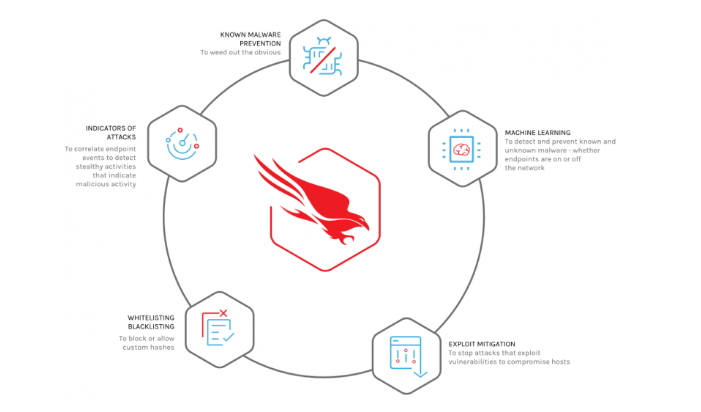
\includegraphics[width=0.9\textwidth]{PhotoMemoire/newgenerationanti.png}
	\caption{Les Différentes Parties Des Antivirus de Nouvelle Génération\cite{15} }
	\end{center}
\end{figure}

\begin{enumerate}
 

 \item  Prévention des logiciels malveillants connus et inconnus
\subitem{a)} Protection antimalware sans fichiers de signatures
 La protection antimalware sans fichiers de signatures utilise des algorithmes de Machine Learning pour déterminer la probabilité qu’un fichier soit malveillant. Les nouvelles menaces sont bloquées en temps réel et la rentabilité est immédiate.
 
 \subitem{b)} Machine Learning
 Le Machine Learning peut détecter et contrer les logiciels malveillants connus et inconnus, que les endpoints soient connectés au réseau ou non. Il détecte les indicateurs d’attaque de manière plus rapide et précise, élimine les ransomwares et comble les failles laissées par les antivirus d’ancienne génération.
 
\item  Prévention des attaques sans logiciels malveillants
 \subitem{a)}. Indicateurs d’attaque
 Les indicateurs d’attaque mettent en corrélation les événements se produisant au niveau des endpoints afin de détecter les activités furtives, signes d’intentions malveillantes.\\ 
 Une solution s’appuyant sur une analyse hors ligne rétrospective pour identifier les indicateurs d’attaque est incapable de rester au fait des dernières cybermenaces, en plus de nécessiter des ressources considérables.\\
  Les algorithmes en ligne qui exploitent le Machine Learning et n’ont pas besoin d’un ensemble complet de données pour effectuer des analyses pertinentes sont à la fois plus rapides, plus efficaces et plus performants.\\
 
 \subitem{b)} Blocage des exploits
 Les malwares ne sont pas toujours distribués au moyen de fichiers. Les attaques basées sur des macros, des commandes d’exécution, des chargeurs en mémoire et d’autres techniques sans fichiers sont en effet de plus en plus courantes.\\
  Le blocage des exploits permet de détecter et de bloquer les exploits dès qu’ils se produisent.\\
 
 \item Intégration de la cyberveille
 L’intégration de la cyberveille permet de déterminer immédiatement l’origine, l’impact et la gravité des attaques dans l’environnement et apporte les conseils nécessaires pour une intervention décisive et une résolution rapide.\\
 
 \item Solution native au cloud
 L’architecture cloud est une composante fondamentale des antivirus de nouvelle génération.\\
  Un NGAV basé dans le cloud peut être totalement opérationnel en quelques secondes, et ce sans redémarrage, mise à jour des signatures, configuration ni acquisition d’une nouvelle infrastructure.\\
   Les algorithmes peuvent traiter en direct l’activité des endpoints et exposer les fichiers malveillants et les comportements suspects en temps quasi réel, sans incidence sur les performances des endpoints.\\
\end{enumerate}

\section{Bonnes pratiques en matière de sécurité informatique}

La prévalence du terme « \textbf{sécurité informatique} » ne signifie nullement que la sécurité est un « \textbf{problème informatique }». Ce n’est pas non plus un problème qui sera résolu uniquement à l’aide de solutions technologiques.\\ Pour élaborer une stratégie de cybersécurité à la fois complète et efficace, les entreprises doivent tenir compte des règles, des processus et des technologies mis en œuvre dans l’ensemble des fonctions métier.\\ Par ailleurs, les utilisateurs du réseau doivent être correctement formés aux comportements responsables en ligne, ainsi qu’à la détection des signes d’attaques réseau courantes.\\
Dans le monde connecté actuel, une stratégie de cybersécurité globale est absolument essentielle. Les stratégies de cybersécurité les plus efficaces combinent ressources humaines et solutions technologiques avancées, telles que l’intelligence artificielle (IA), le Machine Learning (ML) et d’autres formes d’automatisation intelligente, afin d’améliorer la détection des activités anormales et de réduire le délai d’intervention et de correction.\\



